\documentclass[12pt,a4paper]{report}
\usepackage[utf8]{inputenc}
\usepackage{amsmath,amssymb}
\usepackage{lipsum} % for dummy text; remove in final version
\usepackage{minted}
\usepackage[many]{tcolorbox}
\usepackage{xcolor}
\usepackage{pgfplots}
\usepackage{hyperref}
\pgfplotsset{compat=1.18}


\definecolor{main}{HTML}{5989cf}    % setting main color to be used
\definecolor{sub}{HTML}{F2FFF2}     % setting sub color to be used

\tcbset{
    sharp corners,
    colback = white,
    before skip = 0.2cm,    % add extra space before the box
    after skip = 0.5cm      % add extra space after the box
}                           % setting global options for tcolorbox
\newtcolorbox{boxC}{
    colback = sub, % background color
    boxrule = 0pt  % no borders
}
\hypersetup{
    colorlinks=true,
    linkcolor=blue,
    urlcolor=cyan,
    pdftitle={Encrypting Equations Project},
    pdfauthor={Your Name},
}

\begin{document}

\title{
    \Huge\bfseries Encrypting Equations\\[1em]
    \large A Group Project Report
}
\author{SciMathSoc
\vspace{1em}\\IIT Kanpur}
\date{\today}


% Title page
\maketitle
\thispagestyle{empty}
\clearpage

% Table of contents
\tableofcontents
\clearpage

% Chapter 1
\chapter{Introduction}
\section{Motivation}
\section{Objective of the Project}
\section{Outline of the Report}

% Chapter 2
\chapter{Mathematical Prerequisites}

\section{Galois Field Multiplicaation}
In AES, the bytes are treated as elements of the Galois Field \( GF(2^8) \). Each byte corresponds to a polynomial of degree less than 8 with coefficients in \( GF(2) \). For example, the byte \texttt{0x57} (binary: 0101 0111) corresponds to the polynomial:

\[
x^6 + x^4 + x^2 + x + 1
\]

\section*{Irreducible Polynomial}

Multiplication is carried out modulo the irreducible polynomial used in AES:

\[
m(x) = x^8 + x^4 + x^3 + x + 1 \quad \text{(hex: 0x11B)}
\]

This ensures the result of the multiplication remains within the field \( GF(2^8) \).

\section*{Procedure for Galois Field Multiplication}

Let \( a \) and \( b \) be two bytes (i.e., 8-bit values). The goal is to compute:

\[
c = a \cdot b \mod m(x)
\]

The multiplication is done using the \textbf{Russian Peasant Multiplication} algorithm, adapted for \( GF(2^8) \):

\begin{enumerate}
    \item Initialize the result: \( \text{res} = 0 \)
    \item Repeat for 8 iterations:
    \begin{enumerate}
        \item If the least significant bit (LSB) of \( b \) is 1, then:
        \[
        \text{res} = \text{res} \oplus a
        \]
        \item Check if the most significant bit (MSB) of \( a \) is 1:
        \begin{itemize}
            \item If yes: 
            \[
            a = (a \ll 1) \oplus 0x1B
            \]
            \item If no: 
            \[
            a = a \ll 1
            \]
        \end{itemize}
        \item Right shift \( b \): 
        \[
        b = b \gg 1
        \]
    \end{enumerate}
\end{enumerate}

\section*{Explanation}

\begin{itemize}
    \item The bitwise left shift on \( a \) corresponds to multiplying by \( x \) in polynomial form.
    \item If the MSB of \( a \) was 1, then the result would be a degree 8 polynomial and must be reduced modulo \( m(x) \), which is equivalent to XORing with \texttt{0x1B}.
    \item The final result after 8 steps is the product \( a \cdot b \mod m(x) \).
\end{itemize}

\section*{Example}

Let \( a = \texttt{0x57} \), \( b = \texttt{0x83} \):

\begin{itemize}
    \item Convert to binary: \( a = 0101~0111 \), \( b = 1000~0011 \)
    \item Using the procedure above, the multiplication yields: 
    \[
    0x57 \cdot 0x83 = 0xC1
    \]
\end{itemize}

\section*{Summary}

Galois multiplication in AES is not standard integer multiplication. It is a bitwise operation following rules of finite field arithmetic under \( GF(2^8) \), involving:

\begin{itemize}
    \item XOR for addition
    \item Left shifts and conditional reduction for multiplication
    \item Modular reduction using irreducible polynomial \( x^8 + x^4 + x^3 + x + 1 \)
\end{itemize}
\section{Binary Exponentiation}
source to study Binary Exponentiation: \href{https://cp-algorithms.com/algebra/binary-exp.html}{Binary Exponentiation by cp-algorithms}
\newline
\newline
Binary exponentiation is a method used to improve the time-complexity of calculating $a^n$ from $O(n)$(using brute-force multiplication) to $O(\log{n})$.\\
The key idea of BE, is to use the binary representation of the exponent.
consider the integer $n$ and the exponent $a^n$, there are exactly $\lfloor\log_2{n}\rfloor+1$ digits in the binary representation of n, hence we need to perform only $O(\log{n})$ multiplications considering we know the values of:
\[
a, a^2, a^4 ...., a^{2\lfloor\log_2{n}\rfloor}
\]
These values can be found easily by just squaring the previous term, so we get all of these terms with $O(\log{n})$ operations, Finally giving us a time complexity of $O(\log{n})$.
this method can be used for any kind of group operations, which satisfy associative property, for example: elliptic curves.\\
\textbf{Example: }Consider calculating the value of $3^{13}$, with regular multiplication, it will take $O(n)$ operations to get the final answer. So let's use Binary Exp method to find the answer. Consider the Binary representation of the exponent 13:
\[
13 = 1 \cdot 2^0 + 0 \cdot 2^1 + 1 \cdot 2^2 + 1 \cdot 2^3
\]
which gives us:
\[
3^{13} = 3^1 \cdot 3^4 \cdot 3^8
\]
we have to perform only $O(\log{n})$ to get the final answer, considering we know the values of each $3^{2k}$, which is easy to find by squaring the previous term:
\begin{align*}
    3^1 &= 3\\
    3^2 &= 3^1 \cdot 3^1 = 9\\
    3^4 &= 3^2 \cdot 3^2 = 81\\
    3^8 &= 3^4 \cdot 3^4 = 6561
\end{align*}
The final complexity of this algorithm is \textbf{$O(\log{n})$}, we need to compute $\log{n}$ powers of $a$, and then do atmost $\log{n}$ multiplications of these powers.\\
Note that this method can be used to calculate large scalar multiples of point addition $kP$ in elliptic curves, by considering the binary representation of $k$.

\section{The Discrete Logarithm Problem}
Consider a group $G$ and an element $g \in G$. The \textbf{Discrete Logarithm Problem} states that: 
\begin{boxC}
Consider an element $h \in G$ which is generated by $g$, find the integer $n$ satisfying
\[
h = g^n
\]
\end{boxC}

The \textbf{index}(or logarithm) of h with respect to g is defined as the smallest integer n which satisfies \(h = g^n\). It is given by:
\[
n = \log_g{(h)} \quad \text{(or)} \quad n = \text{ind}_g(h)
\]
The \textbf{DLP} is a widely used hard problem in cryptography, we can find its uses in different algorithms like \textbf{Diffie-Hellman key exchange, ELGamal encryption, ECC based algorithms, etc...}\\
We need to be careful about the Group on which we are trying to use the DLP, as for some groups, DLP is very easy for example:
\begin{itemize}
    \item $\mathbb{Z}/m\mathbb{Z}$ under addition operation.
    \item $\mathbb{R}^*$ under multiplication operation.
\end{itemize}
But for the field $\mathbb{F}_p^*$ under multiplication, the DLP is considered to be hard, with the best known algorithm taking \textbf{sub-exponential} time to solve the problem.
\section{Elliptic Curves}
\begin{itemize}
    \item Elliptic curve is an algebraic curve defined by the Weierstrass formula: $y^2 = x^3 + Ax + B$, where A and B are elements of the field over which the elliptic curve is defined.
    \item the EC-equation is supposed to have distinct roots, or you can say the Elliptic curve equation should be \textbf{non singular}, to find if the curve is non-singular or not, we consider the \textbf{Discriminant} of the elliptic curve, which is defined by:
    \[
    \triangle = 4A^3 + 27B^2 \neq 0
    \]
    \item We also define an extra point $\mathcal{O}$ at \textit{infinity}, which acts as the identity element of the groups that we construct using the elliptic curve.
    \item The set of all points we are going to consider is given by:
    \[
    E = \{(x,y) : y^2 = x^3 + Ax+B\} \cup \{\mathcal{O\}}
    \]
\end{itemize}
\section{Elliptic Curves Group Operations}
Let's consider two points P and Q over the elliptic curve, the \textbf{addition} of points P and Q is defined by extending the line passing through PQ, and then reflecting the third point R at which the line intersects the curve about the x-axis.\\
The addition law of E has the following properties:
\begin{enumerate}
    \item $P + \mathcal{O} = \mathcal{O} + P \quad$ for all $P \in E$ (Additive Identity).
    \item $P + (-P) = \mathcal{O} \quad $ for all $P \in E$ (Additive Inverse)
    \item $P+(Q+R) = (P+Q)+R \quad$ for all $P, Q, R \in E$ (Associative Property)
    \item $P+Q = Q+P \quad$ for all $P,Q \in E$ (Commutative Property)
\end{enumerate}
\subsection*{Point Addition Formulas}

Let $E$ be an elliptic curve defined over a field with equation:
\[
E : y^2 = x^3 + ax + b
\]

Let $P = (x_1, y_1)$ and $Q = (x_2, y_2)$ be two points on $E$, and let $R = P + Q = (x_3, y_3)$ be their sum under the group law. The formulas for point addition are as follows:

\begin{itemize}
  \item \textbf{Case 1:} $P \neq Q$ and $x_1 \neq x_2$
  \[
  \lambda = \frac{y_2 - y_1}{x_2 - x_1}, \quad
  x_3 = \lambda^2 - x_1 - x_2, \quad
  y_3 = \lambda(x_1 - x_3) - y_1
  \]

  \item \textbf{Case 2:} $P = Q$ (point doubling) and $y_1 \neq 0$
  \[
  \lambda = \frac{3x_1^2 + a}{2y_1}, \quad
  x_3 = \lambda^2 - 2x_1, \quad
  y_3 = \lambda(x_1 - x_3) - y_1
  \]

  \item \textbf{Case 3:} $P = -Q$ or $P = Q$ and $y_1 = 0$  
  \[
  P + Q = \mathcal{O}
  \]
  (the point at infinity, i.e., the identity element)
\end{itemize}

Here, $\lambda$ denotes the slope of the tangent or secant line used in the addition process.\\
\begin{center}
    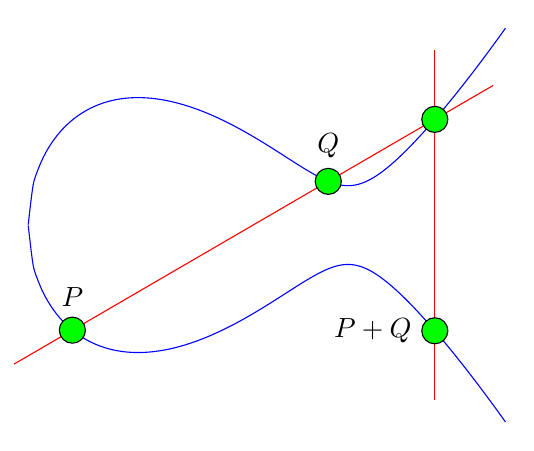
\begin{tikzpicture}[yscale=0.5]
                
			%TODO: up sample size
			\draw[domain=-4.060646:2,samples=100,smooth,variable=\x,blue] plot ({\x},{sqrt(\x^3 + 4*(\x)^2 + 1)});
			\draw[domain=-4.060646:2,samples=100,smooth,variable=\x,blue] plot ({\x},{-sqrt(\x^3 + 4*(\x)^2 + 1)});
			\node (P) at (-3.5, -2.66926956300783) {};
			\node (Q) at (-0.25, 1.1102430216445) {};
			\node (R) at (1.10295826812394, 2.68474117626385) {};
			\node (P+Q) at (1.10295826812394, -2.68474117626385) {};
			\draw[color=red,shorten >=-1cm,shorten <=-1cm] (P) -- (R);
			\draw[color=red,shorten >=-1cm,shorten <=-1cm] (R) -- (P+Q);
			\node[circle,draw=black,fill=green,label=above:{$P$}] at (P) {};
			\node[circle,draw=black,fill=green,label=above:{$Q$}] at (Q) {};
			\node[circle,draw=black,fill=green] at (R) {};
			\node[circle,draw=black,fill=green,label=left:{$P+Q$}] at (P+Q) {};
            
\end{tikzpicture}
\end{center}


\section{Elliptic Curves over \texorpdfstring{$\mathbb{F}_p$}{F_p}}
consider the field $\mathbb{F}_p$ which is defined by:
\[
\mathbb{F}_p = \{0,1, 2, 3 ...., p-1\}
\]
The elliptic curve group defined over $\mathbb{F}_p$ is given by: 
\[
E(\mathbb{F}_p) = \{(x, y): y^2 = x^3 + Ax + B \pmod{p} \quad  \text{with } A,B\in \mathbb{F}_p \} \cup \{\mathcal{O}\}
\]
The addition formulas which were given earlier can be used with the usage of $\pmod{p} $.\\
Let \(P = (x_1,y_1), Q = (x_2,y_2)\in E(\Bbb F_p)\).  Write \(P+Q = R=(x_3,y_3)\).  Then:

\paragraph{Inverse:}
\[
  -P \;=\;(x_1,\,-y_1)\pmod p,
  \quad
  P + (-P) \;=\;\mathcal O.
\]

\paragraph{Addition \((P \neq \pm Q)\):}
\begin{align}
  \lambda &= \frac{y_2 - y_1}{x_2 - x_1} \pmod p, \\
  x_3     &= \lambda^2 - x_1 - x_2 \pmod p, \\
  y_3     &= \lambda\,(x_1 - x_3) - y_1 \pmod p.
\end{align}

\paragraph{Doubling \((P = Q,\;y_1 \neq 0)\):}
\begin{align}
  \lambda &= \frac{3x_1^2 + A}{2\,y_1} \pmod p, \\
  x_3     &= \lambda^2 - 2\,x_1 \pmod p, \\
  y_3     &= \lambda\,(x_1 - x_3) - y_1 \pmod p.
\end{align}

\paragraph{Special cases:}
\begin{itemize}
  \item If \(P = \mathcal O\) then \(P+Q = Q\).
  \item If \(P = (x_1,0)\) then \(P+P = \mathcal O\) (because the tangent is vertical).
\end{itemize}

\section{Elliptic curve Discrete Log problem}
The elliptic curve DLP can be stated as:
\begin{boxC}
    Let $E$ be an elliptic curve defined over $\mathbb{F}_p$.
    \[
    E: y^2 = x^3 + Ax + B \quad A,B \in \mathbb{F}_p.
    \]
    Let $S$ and $T$ be points in $E(\mathbb{F}_p)$, Find an integer $m$, such that:
    \[
    T = mS
    \]
\end{boxC}
We know that m is defined to be the \textbf{index}(or \textbf{logarithm}) of $T$ with respect to $S$.\\
There are different methods to solve the ECDLP, some of them are the exhaustive search method(brute-force method), collision-search method, and most importantly,\textbf{ Pollard's $\rho$ - method}. These methods are not going to be discussed here for now.
Here are some sources to study Pollard's $\rho$ - method:
\begin{itemize}
    \item \href{https://cp-algorithms.com/algebra/factorization.html#pollards-rho-algorithm}{Pollard's rho algorithm - cp-algorithms}
    \item \href{https://en.wikipedia.org/wiki/Pollard%27s_rho_algorithm}{Pollard's rho algorithm - Wikipedia}
\end{itemize}

\section{Basics of Encryption}
Encryption is the process of transforming plaintext into ciphertext so that unauthorized parties cannot read it.  There are two main types of encryption:

\medskip
\noindent\textbf{1. Symmetric (Private‐Key) Encryption.}  
\begin{itemize}
  \item A single secret key \(K\) is shared between sender and receiver.
  \item Encryption: \(C = \mathcal{E}_K(M)\).  
  \item Decryption: \(M = \mathcal{D}_K(C)\).  
  \item Examples: AES, ChaCha20, DES.
  \item Very fast; key‐distribution is the main challenge.
\end{itemize}

\medskip
\noindent\textbf{2. Asymmetric (Public‐Key) Encryption.}  
\begin{itemize}
  \item Key pair \((K_{\text{pub}},K_{\text{priv}})\) with \(K_{\text{pub}}\) publicly known.
  \item Encryption: \(C = \mathcal{E}_{K_{\text{pub}}}(M)\).
  \item Decryption: \(M = \mathcal{D}_{K_{\text{priv}}}(C)\).
  \item Examples: RSA, ElGamal, ECC‐based schemes.
  \item Solves the key‐distribution problem, but slower than symmetric ciphers.
\end{itemize}
% Chapter 3
\chapter{RSA encryption}
sources: \href{https://brilliant.org/wiki/rsa-encryption/}{RSA encryption by Brilliant} and \href{https://en.wikipedia.org/wiki/RSA_cryptosystem#Padding_schemes}{RSA cryptosystem by Wikipedia}.
\section{Key Ideas}
RSA is an example of public key/asymmetric cryptography. There are four key steps to the RSA algorithm.
\begin{enumerate}
    \item key generation
    \item key distribution
    \item encryption
    \item decryption
\end{enumerate}
\section{Key generation and distribution}

    \begin{itemize}
    \item There are two keys that are used in RSA, the \textbf{public key} and the \textbf{private key}. The public key is shared while the private key is only present with the receiver. To create the public key, we first have to choose two really big prime numbers. Usual size of the numbers is around 1024 bits (around 300 digits each), lets say these numbers are $p$ and $q$. We consider their product $n = pq$, as the first half of the public key.
    
    \item The second half of the public key is obtained by using the Euler-totient-function
    \[
        \phi(n) = (p-1) \cdot (q-1)
    \]
    
    \item We find another number $e$ which is \textbf{relatively prime} to $\phi(n)$, usually we choose $e = 2^{16} + 1$ or $e = 3$, we need $e$ to have short-bit length and small \href{https://en.wikipedia.org/wiki/Hamming_weight}{hamming weight}, $e$ forms the second part of our public key.
    
    \item Calculate the multiplicative inverse of $e \pmod{n}$, assume $d$ is the multiplicative inverse of $e$, then we have:
    \[
        d \cdot e \equiv 1 \pmod{n}
    \]
    
    \item $d$ is our \textbf{private key}, this is supposed to be kept secret only with the recipient.
    
    \item Alice shares her public key with Bob through a reliable channel, but doesn't share her private key.
    
    \[
        \text{Alice} \xrightarrow{\text{Public key}} \text{Bob}
    \]
    
    \item Let's say Bob has to send an encrypted message to Alice, Bob needs to know the public key of Alice to encrypt his message, and then he shares his encrypted message to Alice, which is then decrypted by Alice using her private key.
    
    \[
        \text{Bob} \xrightarrow{\text{Encrypted message}} \text{Alice}
    \]
\end{itemize}
\section{Encryption and decryption}
\begin{itemize}
    \item Let's say Bob has a text-message that he wants to encrypt, firstly he needs to convert it into number-format by using common methods like \href{https://en.wikipedia.org/wiki/ASCII}{ASCII}.
    \item Assuming he converted his message into a number m, we need to make sure that m is smaller than n, i.e $m<n$, because if it is not, then the message will be lost when modulo is taken. Hence if m is greater than n, then divide it into smaller blocks, and send the message block wise.
    \item Once we have the message m, to encrypt it, we need to take modulo exponent of m with public key $e$: 
    \[
    m^e \equiv c\pmod{n}
    \]
    where $c$ is our new encrypted message (also known as \textbf{ciphertext}).
    \item This ciphertext is now transferred to Alice, who takes the modular exponent of the ciphertext $c$ with the private key $d$.
    \[
    c^d \equiv m \pmod{n}
    \]
    through which Alice gets the original message back.
\end{itemize}
\section{Implementation}
A very skeletal code for the implementation of RSA is given here, note that the implementation uses the \href{https://en.wikipedia.org/wiki/GNU_Multiple_Precision_Arithmetic_Library}{GNU-MP} library:
\begin{itemize}
    \item \href{https://github.com/Bing-Chilling-07/SciMathSoc-Encrypting-Eqns/blob/88b2d38ba99ae7b23f1a6825a756a4b4e0faa92e/Encryption%20Algorithms/RSA-GMP.c}{RSA-GMP.c}
\end{itemize}
The output of the code is given by(note that we are printing every value only for demonstration):
\begin{minted}[linenos, bgcolor=gray!10, breaklines=true, fontsize=\small]{c}
Primality test passed I guess.
p = 90344467931018478790369878185660823024745220039813
q = 6938869227845931063641427769065486324636885252537479

String_p: 90344467931018478790369878185660823024745220039813
String_q: 6938869227845931063641427769065486324636885252537479 
the value of n is equal to: 62688844843265767309785505463840257866703235290347409601332
9044508728577080168542216780788659654651427
phi(n) is given by: 62688844843265767309785505463840257866703235290346706679963
3267559186145282521291069633127029182074136
e is equal to: 100000000000000000001
gcd of phi(n) and e is equal to: 1
d is equal to: 4396053453892243043222468546530791921138915805645683609195
30371460078820870254707992788128236827797969
Enter maximum string length (make sure len(msg)<n): 10
Enter your string (up to 10 characters): 1234567890
You entered: "1234567890"

your encrypted message is: 1883769588604620013447615371111107418033550137589780582
75426265198927897319336758320824329325608641288
your decrypted message is: 1234567890
\end{minted}


% Chapter 4
\chapter{Diffie Hellman key exchange}
Diffie Hellman key exchange is a symmetric key distribution method, which helps us to share a secret over public channels.
\section{Key Ideas}
\section{Implementation}
\section{Security Aspects}

\chapter{ELGamal Key exchange}
\chapter{AES Encryption}

\section{Introduction}
The Advanced Encryption Standard (AES) is a symmetric block cipher adopted as a standard by NIST in 2001. It encrypts data in fixed blocks of 128 bits using cipher keys of 128, 192, or 256 bits. AES is secure, fast, and suitable for hardware and software implementation.

\section{State Array}
The AES algorithm processes data as a $4 \times 4$ byte matrix known as the \textbf{State}. Each byte is an element of the finite field $\mathbb{F}_{2^8}$.

\section{XOR Operation (Add Round Key)}
AES uses XOR to combine the State with the Round Key.

The XOR is a fast and reversible bitwise operation. It is used in the \texttt{Add Round Key} step.

\section{Galois Field Multiplication}
AES uses multiplication in the Galois Field ($GF(2^8)$), with the irreducible polynomial:
\[
x^8 + x^4 + x^3 + x + 1
\]

This defines how bytes are multiplied. 
\begin{itemize}
    \item Common constants used: 1, 2, 3 (in hexadecimal: 0x01, 0x02, 0x03)
    \item Multiplication is performed modulo the above polynomial.
\end{itemize}

\section{Substitution-Box}
It is a look-up table that helps in transforming one state into another new state in the encryption process.

\section{SubBytes}
Each byte of the State is substituted using a nonlinear S-box derived from the multiplicative inverse in $\mathbb{F}_{2^8}$.

\section{ShiftRows}
AES cyclically shifts each row in the State:
\begin{itemize}
\item Row 0: no shift
\item Row 1: left shift by 1 unit
\item Row 2: left shift by 2 units
\item Row 3: left shift by 3 units
\end{itemize}

\section{MixColumns}
Each column is treated as a 4-byte vector and multiplied by a fixed matrix over $GF(2^8)$, given by:
\[
\begin{bmatrix}
d_0 \\
d_1 \\         
d_2 \\
d_3
\end{bmatrix}
=
\begin{bmatrix}
2 & 3 & 1 & 1 \\
1 & 2 & 3 & 1 \\         
1 & 1 & 2 & 3 \\
3 & 1 & 1 & 2
\end{bmatrix}
\begin{bmatrix}
b_0 \\
b_1 \\         
b_2 \\
b_3
\end{bmatrix}
\]

\section{Round Keys and Key Expansion}
AES expands the cipher key into an array of words. So, it gets expanded to 11 rounds from 10 rounds. Each round uses 4 words (16 bytes). Each round key expansion uses:
\begin{itemize}
\item \textbf{RotWord}: Rotates a 4-byte word left by 1 unit.
\item \textbf{SubWord}: Substitutes a 4-byte word using S-box on each byte.
\item \textbf{Rcon}: Denotes round constants which are added to the subword.
\end{itemize}

\subsection{Round Constants (Rcon)}
Round constants are derived from powers of 2 in $GF(2^8)$.\\
They are defined recursively as:
\[
\begin{aligned}
rc(1) &= 1 \\
rc(i) &= 2 \cdot rc(i-1), \quad \text{if } rc(i-1) < 0x80 \\
rc(i) &= 2 \cdot rc(i-1) \oplus 0x11B, \quad \text{if } rc(i-1) \ge 0x80
\end{aligned}
\]
Each Rcon is XOR'ed to the first byte of the round key.

\subsection{Key Expansion Procedure (128-bit)}
Each round key is passed through \textbf{RotWord}, then passed through \textbf{SubWord}, and finally \textbf{Rcon} is added.\\
Columns of next round key are obtained through addition of the previous column of the same round key and the corresponding column in the previous round key.
\begin{figure}[H]
    \centering
    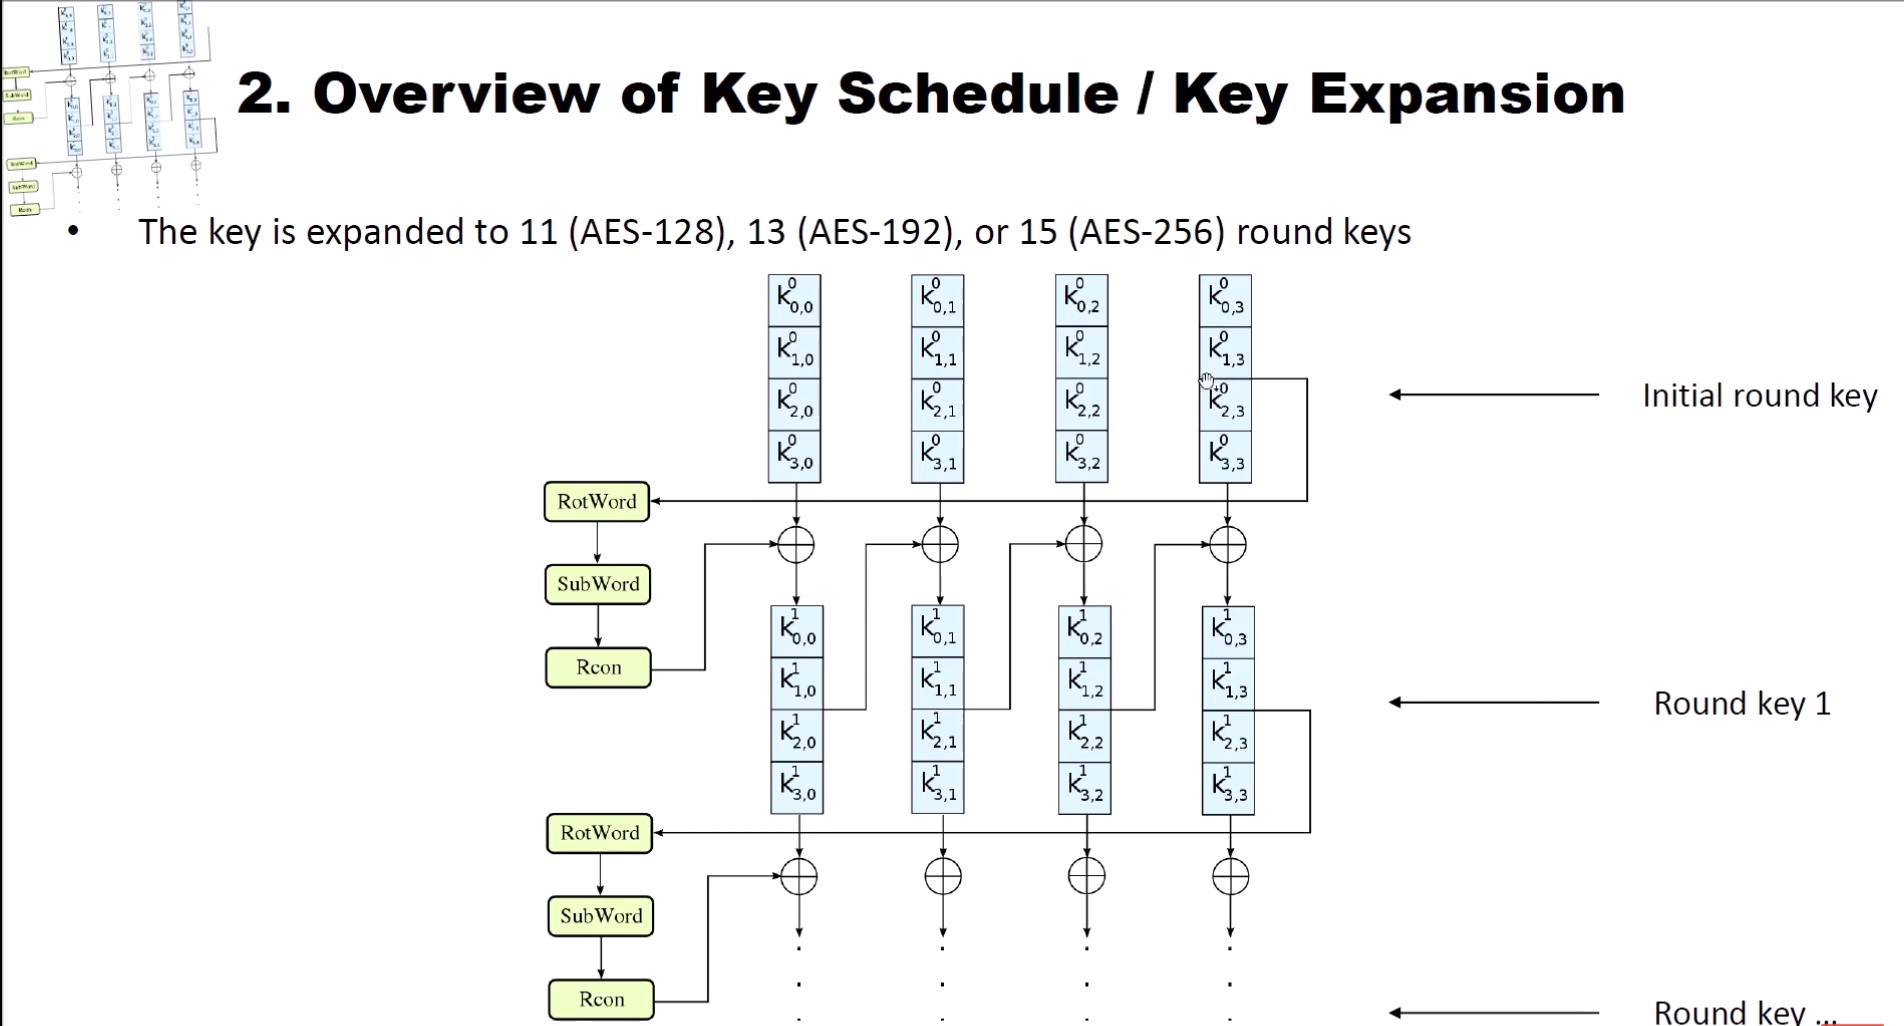
\includegraphics[width=0.5\textwidth]{screenshot.png}
    \caption{AES-128 Algorithm}
\end{figure}

\section{Encryption Procedure}
AES encryption consists of the following steps for a 128-bit key:
\begin{enumerate}
\item \textbf{Initial Round}:
\begin{itemize}
\item AddRoundKey(State, RoundKey)
\end{itemize}

\item \textbf{Main Rounds (9 rounds)}:\\
For round $r = 1$ to $9$:
\begin{itemize}
    \item SubBytes(State)
    \item ShiftRows(State)
    \item MixColumns(State)
    \item AddRoundKey(State, RoundKey)
\end{itemize}

\item \textbf{Final Round (10th)}:
\begin{itemize}
    \item SubBytes(State)
    \item ShiftRows(State)
    \item AddRoundKey(State, RoundKey)
\end{itemize}

\item The output is the ciphertext (final State matrix converted to bytes).
\end{enumerate}

\section{Decryption Procedure}
The decryption process of AES is the inverse of encryption and consists of:
\begin{enumerate}
\item \textbf{Initial Round (10th)}:
\begin{itemize}
\item AddRoundKey(State, RoundKey)
\end{itemize}

\item \textbf{Main Rounds (9 rounds)}:\\
For round $r = 9$ to $1$:
\begin{itemize}
    \item InvShiftRows(State)
    \item InvSubBytes(State)
    \item AddRoundKey(State, RoundKey)
    \item InvMixColumns(State)
\end{itemize}

\item \textbf{Final Round (0th)}:
\begin{itemize}
    \item InvShiftRows(State)
    \item InvSubBytes(State)
    \item AddRoundKey(State, RoundKey)
\end{itemize}

\item The output is the original plaintext.
\end{enumerate}

The inverse operations (\texttt{InvSubBytes}, \texttt{InvShiftRows}, \texttt{InvMixColumns}) use corresponding inverse S-box and transformations in $GF(2^8)$.

\section{Resources}
\href{https://colab.research.google.com/drive/1xG7OrAtUqqsfvo9QRrrAGK-PmNgoB5Zf#scrollTo=ioJzVTF3HBwT}{AES-128 Algorithm}\\
\href{https://youtu.be/h6wvqm0aXco?si=lmESeaAiUIHnJjqN}{AES – The Advanced Encryption Standard Explained}\\
\href{https://youtu.be/rmqWaktEpcw?si=qunMHYUmwdtMGwfW}{AES – Key Schedule/Key Expansion Explained}

%Chapter 6
\chapter{Primality testing}
\section{Miller Rabin primality test}

% Chapter 6
\chapter{Conclusion}
\section{Summary}
\section{Future Work}
\section{References}

% Bibliography (optional)
% \bibliographystyle{plain}
% \bibliography{references}

\end{document}

